\documentclass[11pt,twoside,letterpaper]{article}
\newcommand{\reporttitle}{Lab 4: Path Planning with A* on a SLAM Map}
\newcommand{\reportauthorOne}{Adams, Hunter}
\newcommand{\cidOne}{20997503}
\newcommand{\reportauthorTwo}{Chen, Joe}
\newcommand{\cidTwo}{20998545}
\newcommand{\reportauthorThree}{Wielowieyski, Jacob}
\newcommand{\cidThree}{21004619}
\newcommand{\robotNumber}{7}     % TODO check: robot used in lab 4
\newcommand{\stationNumber}{151} % TODO check: station used in lab 4
\date{\today}
%%%%%%%%%%%%%%%%%%%%%%%%%%%%%%%%%%%%%%%%%
% University Assignment Title Page 
% LaTeX Template
% Version 1.0 (27/12/12)
%
% This template has been downloaded from:
% http://www.LaTeXTemplates.com
%
% Original author:
% WikiBooks (http://en.wikibooks.org/wiki/LaTeX/Title_Creation)
%
% License:
% CC BY-NC-SA 3.0 (http://creativecommons.org/licenses/by-nc-sa/3.0/)
% 
% Instructions for using this template:
% This title page is capable of being compiled as is. This is not useful for 
% including it in another document. To do this, you have two options: 
%
% 1) Copy/paste everything between \begin{document} and \end{document} 
% starting at \begin{titlepage} and paste this into another LaTeX file where you 
% want your title page.
% OR
% 2) Remove everything outside the \begin{titlepage} and \end{titlepage} and 
% move this file to the same directory as the LaTeX file you wish to add it to. 
% Then add \input{./title_page_1.tex} to your LaTeX file where you want your
% title page.
%
%----------------------------------------------------------------------------------------
%	PACKAGES AND OTHER DOCUMENT CONFIGURATIONS
%----------------------------------------------------------------------------------------
\usepackage{ifxetex}
\usepackage{textpos}
\usepackage{natbib}
\usepackage{kpfonts}
\usepackage[letterpaper,hmargin=2.8cm,vmargin=2.0cm,includeheadfoot]{geometry}
\usepackage{ifxetex}
\usepackage{stackengine}
\usepackage{tabularx,longtable,multirow,subfigure,caption}%hangcaption
\usepackage{fncylab} %formatting of labels
\usepackage{fancyhdr}
\usepackage{color}
\usepackage[tight,ugly]{units}
\usepackage{url}
\usepackage{float}
\usepackage[english]{babel}
\usepackage{amsmath}
\usepackage{graphicx}
\usepackage[colorinlistoftodos]{todonotes}
\usepackage{dsfont}
\usepackage{epstopdf} % automatically replace .eps with .pdf in graphics
\usepackage{natbib}
\usepackage{backref}
\usepackage{array}
\usepackage{latexsym}
\usepackage{etoolbox}

\usepackage{enumerate} % for numbering with [a)] format 



\ifxetex
\usepackage{fontspec}
\setmainfont[Scale=.8]{OpenDyslexic-Regular}
\else
\usepackage[pdftex,pagebackref,hypertexnames=false,colorlinks]{hyperref} % provide links in pdf
\hypersetup{pdftitle={},
  pdfsubject={}, 
  pdfauthor={\reportauthorOne},
  pdfkeywords={}, 
  pdfstartview=FitH,
  pdfpagemode={UseOutlines},% None, FullScreen, UseOutlines
  bookmarksnumbered=true, bookmarksopen=true, colorlinks,
    citecolor=black,%
    filecolor=black,%
    linkcolor=black,%
    urlcolor=black}
\usepackage[all]{hypcap}
\fi

\usepackage{tcolorbox}

% various theorems
\usepackage{ntheorem}
\theoremstyle{break}
\newtheorem{lemma}{Lemma}
\newtheorem{theorem}{Theorem}
\newtheorem{remark}{Remark}
\newtheorem{definition}{Definition}
\newtheorem{proof}{Proof}

% example-environment
\newenvironment{example}[1][]
{ 
\vspace{4mm}
\noindent\makebox[\linewidth]{\rule{\hsize}{1.5pt}}
\textbf{Example #1}\\
}
{ 
\noindent\newline\makebox[\linewidth]{\rule{\hsize}{1.0pt}}
}



%\renewcommand{\rmdefault}{pplx} % Palatino
% \renewcommand{\rmdefault}{put} % Utopia

\ifxetex
\else
\renewcommand*{\rmdefault}{bch} % Charter
\renewcommand*{\ttdefault}{cmtt} % Computer Modern Typewriter
%\renewcommand*{\rmdefault}{phv} % Helvetica
%\renewcommand*{\rmdefault}{iwona} % Avant Garde
\fi

\setlength{\parindent}{0em}  % indentation of paragraph

\setlength{\headheight}{14.5pt}
\pagestyle{fancy}
\fancyfoot[ER,OL]{\thepage}%Page no. in the left on
                                %odd pages and on right on even pages
\fancyfoot[OC,EC]{\sffamily }
\renewcommand{\headrulewidth}{0.1pt}
\renewcommand{\footrulewidth}{0.1pt}
\captionsetup{margin=10pt,font=small,labelfont=bf}


%--- chapter heading

\def\@makechapterhead#1{%
  \vspace*{10\p@}%
  {\parindent \z@ \raggedright %\sffamily
        %{\Large \MakeUppercase{\@chapapp} \space \thechapter}
        %\\
        %\hrulefill
        %\par\nobreak
        %\vskip 10\p@
    \interlinepenalty\@M
    \Huge \bfseries 
    \thechapter \space\space #1\par\nobreak
    \vskip 30\p@
  }}

%---chapter heading for \chapter*  
\def\@makeschapterhead#1{%
  \vspace*{10\p@}%
  {\parindent \z@ \raggedright
    \sffamily
    \interlinepenalty\@M
    \Huge \bfseries  
    #1\par\nobreak
    \vskip 30\p@
  }}
  



% %%%%%%%%%%%%% boxit
\def\Beginboxit
   {\par
    \vbox\bgroup
	   \hrule
	   \hbox\bgroup
		  \vrule \kern1.2pt %
		  \vbox\bgroup\kern1.2pt
   }

\def\Endboxit{%
			      \kern1.2pt
		       \egroup
		  \kern1.2pt\vrule
		\egroup
	   \hrule
	 \egroup
   }	

\newenvironment{boxit}{\Beginboxit}{\Endboxit}
\newenvironment{boxit*}{\Beginboxit\hbox to\hsize{}}{\Endboxit}



\allowdisplaybreaks

\makeatletter
\newcounter{elimination@steps}
\newcolumntype{R}[1]{>{\raggedleft\arraybackslash$}p{#1}<{$}}
\def\elimination@num@rights{}
\def\elimination@num@variables{}
\def\elimination@col@width{}
\newenvironment{elimination}[4][0]
{
    \setcounter{elimination@steps}{0}
    \def\elimination@num@rights{#1}
    \def\elimination@num@variables{#2}
    \def\elimination@col@width{#3}
    \renewcommand{\arraystretch}{#4}
    \start@align\@ne\st@rredtrue\m@ne
}
{
    \endalign
    \ignorespacesafterend
}
\newcommand{\eliminationstep}[2]
{
    \ifnum\value{elimination@steps}>0\leadsto\quad\fi
    \left[
        \ifnum\elimination@num@rights>0
            \begin{array}
            {@{}*{\elimination@num@variables}{R{\elimination@col@width}}
            |@{}*{\elimination@num@rights}{R{\elimination@col@width}}}
        \else
            \begin{array}
            {@{}*{\elimination@num@variables}{R{\elimination@col@width}}}
        \fi
            #1
        \end{array}
    \right]
    & 
    \begin{array}{l}
        #2
    \end{array}
    &%                                    moved second & here
    \addtocounter{elimination@steps}{1}
}
\makeatother

%% Fast macro for column vectors
\makeatletter  
\def\colvec#1{\expandafter\colvec@i#1,,,,,,,,,\@nil}
\def\colvec@i#1,#2,#3,#4,#5,#6,#7,#8,#9\@nil{% 
  \ifx$#2$ \begin{bmatrix}#1\end{bmatrix} \else
    \ifx$#3$ \begin{bmatrix}#1\\#2\end{bmatrix} \else
      \ifx$#4$ \begin{bmatrix}#1\\#2\\#3\end{bmatrix}\else
        \ifx$#5$ \begin{bmatrix}#1\\#2\\#3\\#4\end{bmatrix}\else
          \ifx$#6$ \begin{bmatrix}#1\\#2\\#3\\#4\\#5\end{bmatrix}\else
            \ifx$#7$ \begin{bmatrix}#1\\#2\\#3\\#4\\#5\\#6\end{bmatrix}\else
              \ifx$#8$ \begin{bmatrix}#1\\#2\\#3\\#4\\#5\\#6\\#7\end{bmatrix}\else
                 \PackageError{Column Vector}{The vector you tried to write is too big, use bmatrix instead}{Try using the bmatrix environment}
              \fi
            \fi
          \fi
        \fi
      \fi
    \fi
  \fi 
}  
\makeatother

\robustify{\colvec}

%%% Local Variables: 
%%% mode: latex
%%% TeX-master: "notes"
%%% End: 

% quick way of adding a figure
\newcommand{\fig}[3]{
 \begin{center}
 \scalebox{#3}{\includegraphics[#2]{#1}}
 \end{center}
}

%\newcommand*{\point}[1]{\vec{\mkern0mu#1}}
\newcommand{\ci}[0]{\perp\!\!\!\!\!\perp} % conditional independence
\newcommand{\point}[1]{{#1}} % points 
\renewcommand{\vec}[1]{{\boldsymbol{{#1}}}} % vector
\newcommand{\mat}[1]{{\boldsymbol{{#1}}}} % matrix
\newcommand{\R}[0]{\mathds{R}} % real numbers
\newcommand{\Z}[0]{\mathds{Z}} % integers
\newcommand{\N}[0]{\mathds{N}} % natural numbers
\newcommand{\nat}[0]{\mathds{N}} % natural numbers
\newcommand{\Q}[0]{\mathds{Q}} % rational numbers
\ifxetex
\newcommand{\C}[0]{\mathds{C}} % complex numbers
\else
\newcommand{\C}[0]{\mathds{C}} % complex numbers
\fi
\newcommand{\tr}[0]{\text{tr}} % trace
\renewcommand{\d}[0]{\mathrm{d}} % total derivative
\newcommand{\inv}{^{-1}} % inverse
\newcommand{\id}{\mathrm{id}} % identity mapping
\renewcommand{\dim}{\mathrm{dim}} % dimension
\newcommand{\rank}[0]{\mathrm{rk}} % rank
\newcommand{\determ}[1]{\mathrm{det}(#1)} % determinant
\newcommand{\scp}[2]{\langle #1 , #2 \rangle}
\newcommand{\kernel}[0]{\mathrm{ker}} % kernel/nullspace
\newcommand{\img}[0]{\mathrm{Im}} % image
\newcommand{\idx}[1]{{(#1)}}
\DeclareMathOperator*{\diag}{diag}
\newcommand{\E}{\mathds{E}} % expectation
\newcommand{\var}{\mathds{V}} % variance
\newcommand{\gauss}[2]{\mathcal{N}\big(#1,\,#2\big)} % gaussian distribution N(.,.)
\newcommand{\gaussx}[3]{\mathcal{N}\big(#1\,|\,#2,\,#3\big)} % gaussian distribution N(.|.,.)
\newcommand{\gaussBig}[2]{\mathcal{N}\left(#1,\,#2\right)} % see above, but with brackets that adjust to the height of the arguments
\newcommand{\gaussxBig}[3]{\mathcal{N}\left(#1\,|\,#2,\,#3\right)} % see above, but with brackets that adjust to the height of the arguments
\DeclareMathOperator{\cov}{Cov} % covariance (matrix) 
\ifxetex
\renewcommand{\T}[0]{^\top} % transpose
\else
\newcommand{\T}[0]{^\top}
\fi
% matrix determinant
\newcommand{\matdet}[1]{
\left|
\begin{matrix}
#1
\end{matrix}
\right|
}



%%% various color definitions
\definecolor{darkgreen}{rgb}{0,0.6,0}

\newcommand{\blue}[1]{{\color{blue}#1}}
\newcommand{\red}[1]{{\color{red}#1}}
\newcommand{\green}[1]{{\color{darkgreen}#1}}
\newcommand{\orange}[1]{{\color{orange}#1}}
\newcommand{\magenta}[1]{{\color{magenta}#1}}
\newcommand{\cyan}[1]{{\color{cyan}#1}}


% redefine emph
\renewcommand{\emph}[1]{\blue{\bf{#1}}}

% place a colored box around a character
\gdef\colchar#1#2{%
  \tikz[baseline]{%
  \node[anchor=base,inner sep=2pt,outer sep=0pt,fill = #2!20] {#1};
    }%
}%

\usepackage{booktabs}
\geometry{left=0.7in,right=0.7in,top=0.55in,bottom=0.55in,headheight=14.5pt,headsep=10pt,footskip=20pt}
\setlength{\headwidth}{\textwidth}
\setlength{\parindent}{0pt}
\setlength{\parskip}{3pt}
\setlength{\textfloatsep}{6pt}
\setlength{\floatsep}{6pt}
\setlength{\intextsep}{5pt}
\setlength{\abovedisplayskip}{4pt}\setlength{\belowdisplayskip}{4pt}
\captionsetup{margin=0pt,font=small,labelfont=bf,skip=3pt}
\renewcommand{\topfraction}{0.95}\renewcommand{\bottomfraction}{0.95}\renewcommand{\textfraction}{0.03}\renewcommand{\floatpagefraction}{0.9}
\makeatletter
\renewcommand{\section}{\@startsection{section}{1}{0pt}{7pt}{4pt}{\large\bfseries}}
\makeatother
\newcommand{\para}[1]{\textbf{#1}\quad}
\newcommand{\TODO}[1]{\textcolor{red}{\textbf{TODO:} #1}}   % delete every \TODO before submitting
\fancyhf{}
\fancyhead[LO,LE]{\small MTE544 -- Lab 4}
\fancyhead[RO,RE]{\small Path Planning with A*}
\fancyfoot[CO,CE]{\small \thepage}
\hypersetup{pdftitle={MTE544 Lab 4: Path Planning with A*},pdfauthor={Hunter Adams, Joe Chen, Jacob Wielowieyski}}
\begin{document}
\begin{titlepage}
\thispagestyle{empty}
\begin{center}
\vspace*{0.9cm}

\includegraphics[width=10cm]{figures/uw.png}\\[1.8cm]
{\Large\bfseries MTE544 -- Autonomous Mobile Robotics}\\[0.5cm]
{\large University of Waterloo}\\[0.2cm]
Department of Mechanical and Mechatronics Engineering\\[1.3cm]
\rule{\linewidth}{0.5mm}\\[0.4cm]
{\huge\bfseries \reporttitle\par}
\vspace{0.4cm}
\rule{\linewidth}{0.5mm}
\vspace{1.2cm}

\renewcommand{\arraystretch}{1.35}
\begin{tabular}{ll}
\textbf{Group member (Family Name, First Name)} & \textbf{Student ID}\\
\reportauthorOne & \cidOne\\
\reportauthorTwo & \cidTwo\\
\reportauthorThree & \cidThree\\
\end{tabular}

\vspace{0.9cm}
\begin{tabular}{ll}
\textbf{Station number:} & \stationNumber\\[0.2cm]
\textbf{Robot number:} & \robotNumber
\end{tabular}
\vfill
\makeatletter
\@date
\makeatother
\vspace{0.8cm}
\end{center}
\end{titlepage}

\setcounter{page}{1}
\pagestyle{fancy}

\TODO{Check the Lab 4 handout/rubric on LEARN and rename or reorder the sections below to match it.}

%=====================================================================================================
\section{Map of the room (Part 3)}

The map was built with SLAM toolbox on the TurtleBot~4, driving with teleop from our start mark on the tape, and saved with \texttt{map\_saver\_cli}, and the turtlebot3 cartographer.

\begin{figure}[H]
  \centering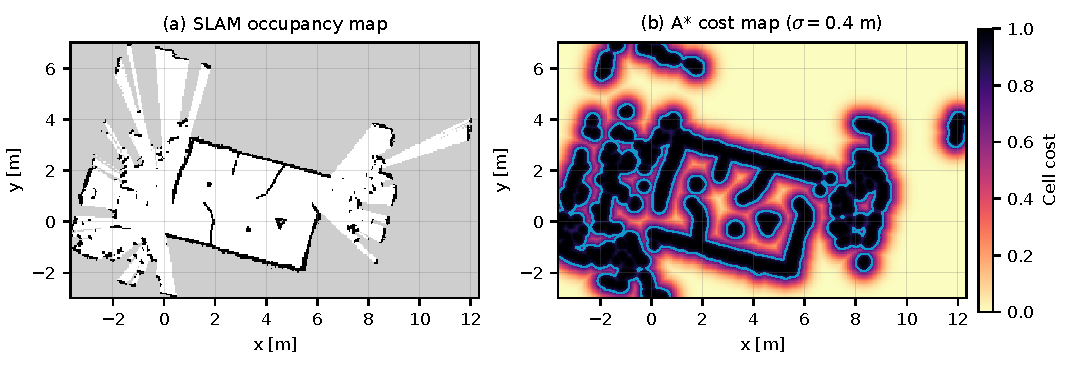
\includegraphics[width=\textwidth]{figures/fig_map.pdf}
  \caption{(a) Occupancy map from SLAM (black: occupied, white: free, grey: unknown).
  (b) Cost map used by A*: a Gaussian of each cell's distance to the nearest obstacle, $\sigma=0.4$\,m. Cells with cost $>0.8$ (inside the blue contour) are treated as walls.}
  \label{fig:map}
\end{figure}
\TODO{comment on map quality, variation in sigma}
%=====================================================================================================
\section{A* and the cost map (Parts 4--5)}

\para{A*.} Search on the cost-map grid, 8-connected. Each node keeps $g$ (cost from the start), $h$ (heuristic to goal, in cells) and $f=g+h$; the open node with the lowest $f$ is expanded next. Moving to cell $n'$ costs the step length plus that cell's cost-map value:
\begin{equation*}
g(n')=g(n)+\underbrace{\{1,\sqrt2\}}_{\text{straight, diagonal}}+c(n'),\qquad
h_{\text{euclidean}}=\sqrt{\Delta x^2+\Delta y^2},\qquad h_{\text{manhattan}}=|\Delta x|+|\Delta y|
\end{equation*}
\TODO{Euclidean never overestimates, manhatten can, Manhatten can lead to going closer to walls in instances with large heurstic costs}

\para{Cost map.} $c(d)=\exp\!\left(-d^2/2\sigma^2\right)$, with $d$ the distance to the nearest occupied cell.
$c>0.8$ for $d<\sigma\sqrt{2\ln1.25}\approx0.67\sigma$.
We raised $\sigma$ from 0.3 to 0.4\,m in lab, so the blocked band grew from 0.20 to 0.27\,m.

\para{Settings carried over.}
\begin{itemize}\setlength\itemsep{0pt}
  \item Localization: EKF from Lab~3, $\mat{R}=\mathrm{diag}(2\times10^{-5},\,2\times10^{-4},\,0.05,\,0.06)$, $\mat{Q}$ raised from $0.25\,\mat{I}$ to $0.375\,\mat{I}$ in lab. Measured from uncertainty in respective sensors.
  \item Trajectory controller (Lab~2): $k_{p}=0.2,\ k_{d}=0.05,\ k_{i}=0.025$ (linear), $k_{p}=1.0,\ k_{d}=0.2,\ k_{i}=0.025$ (angular).
  \item Goal reached when the EKF position is within 5\,cm of the last path point.
\end{itemize}

%=====================================================================================================
\section{Results}

\para{Robot runs (Fig.~\ref{fig:runs}).} Both runs start at the tape mark, use the Euclidean heuristic and the EKF, with the goal set by 2D Goal Pose in RViz.
The EKF stopped within the 5\,cm threshold of the goal, and the odometry agrees within 1.2--1.4\,cm.

\begin{figure}[H]
  \centering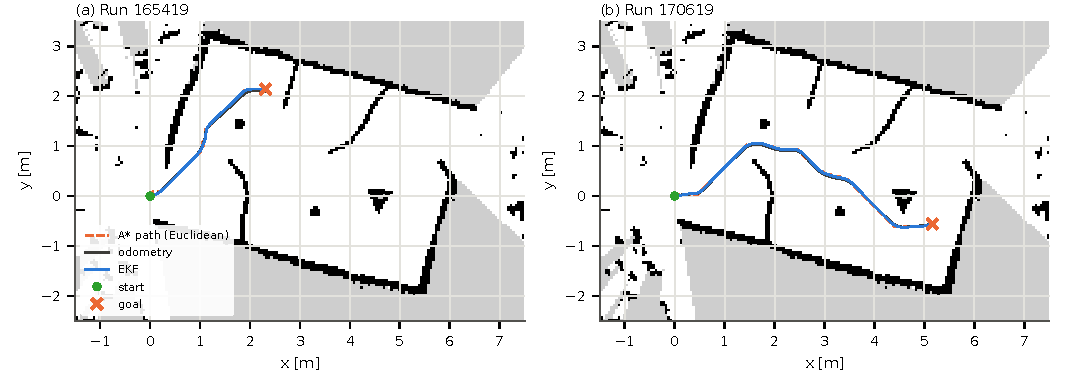
\includegraphics[width=\textwidth]{figures/fig_runs.pdf}
  \caption{The two runs that reached their goal, cut at the goal. (a) 3.45\,m path, goal reached after 289\,s. (b) 6.34\,m path, goal reached after 77\,s.
  EKF and odometry stay within 6\,cm of each other and follow the planned path closely. \TODO{comment on corner cutting / overshoot at turns.}}
  \label{fig:runs}
\end{figure}

\para{Heuristics (Fig.~\ref{fig:heur}).} Only the Euclidean heuristic was driven. To compare, the start and goal of both runs were planned again offline with \texttt{planner.py} (same map, same cost map, $\sigma=0.4$\,m) using each heuristic.
The Euclidean paths are identical, cell for cell, to the ones the robot followed, so the offline planner matches what the robot ran.

\begin{figure}[H]
  \centering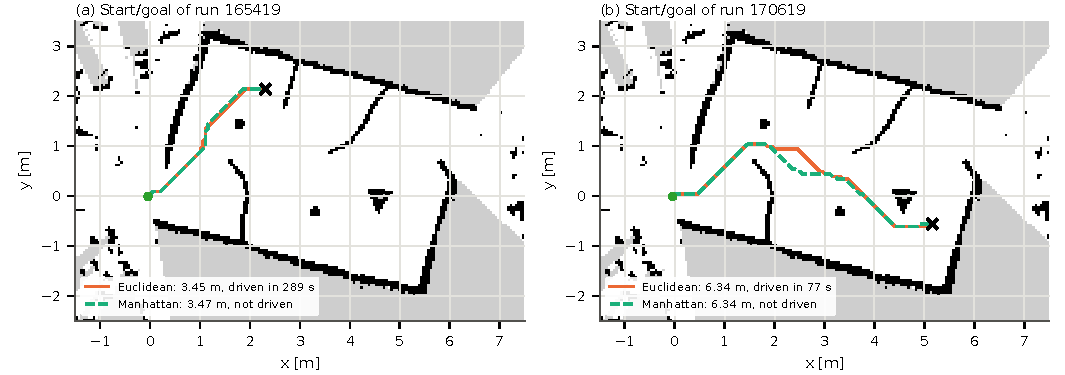
\includegraphics[width=\textwidth]{figures/fig_heuristics.pdf}
  \caption{A* paths from \texttt{planner.py} for both heuristics, with path length and the robot's time to completion (Euclidean only; Manhattan was not driven).
  (a) Manhattan takes a slightly different route near $(1.1,1.2)$\,m. (b) Same length, but Manhattan cuts closer to the wall at $(2.5,0.5)$\,m.}
  \label{fig:heur}
\end{figure}

\begin{table}[H]\centering\small
\caption{Path length per heuristic and time to completion on the robot, numbers from \texttt{report/figures/numbers.json}.}
\begin{tabular}{llrr}\toprule
Goal & Heuristic & Path length [m] & Time to completion [s]\\\midrule
(a) $(2.31,2.14)$ & Euclidean & 3.45 & 289\\
                  & Manhattan & 3.47 & not driven\\
(b) $(5.16,-0.56)$ & Euclidean & 6.34 & 77\\
                   & Manhattan & 6.34 & not driven\\\bottomrule
\end{tabular}
\label{tab:heur}
\end{table}

%=====================================================================================================
\section{Discussion}

\para{Euclidean vs.\ Manhattan.} Manhatten and Euclidean both result in similar distances in operational distance and time, but Manhatten tries to reduce the larger heuristic cost and leads to veering closer to walls and obstacles, which for this applciation is undesireable. 
With diagonal moves Manhattan overestimates the remaining cost (a diagonal step costs $\sqrt2$, Manhattan counts 2), so A* pushes harder toward the goal and can stop at a path that is not the cheapest. Euclidean never overestimates, so its path is optimal for this cost map, at the price of searching more nodes.
On this map both plan in neglibile time, so the speed-up does not matter here; it would on a larger map or with frequent replanning.

\para{Effect of the cost map.}

\para{Localization.} 

\para{Limitations and improvements.}

\end{document}
